\chapter{Rational Functions}
%\addcontentsline{toc}{chapter}{1 Graphs}
%%%%%%%%%%%%%%% SECTION HEADER %%%%%%%%%%%%%%%%
\rhead{2}
\lhead{Rational Functions}
%%%%%%%%%%%%%%%%%%% START %%%$%%%%%%%%%%%%%%%%%
\section{Introduction}
$f(x)$ is a rational function if \[
            f(x) = \frac{p(x)}{q(x)}
\]
where $p(x)$ and $q(x)$ are both a polynomial and $q(x) \neq0$.Here are some examples of rational functions:
\begin{align*}
            f(x) &= \frac{1}{x+4}\\
            g(x) &= \frac{x-3}{x+2}\\
            h(x) &= \frac{x-12}{x^2-2x+3}\\
                 &\vdots
\end{align*}
\section{Domain of a rational function}
As we discussed in previous chapter, when we have a division the denominator cannot be equal to 0. Therefore, domain  of  the  rational  function  consists  of  all  real  numbers  except  the  zeros  of  the  denominator.
% ===== EXAMPLE 1
\begin{exa}
        Find the domain of each rational functions:
        \begin{enumerate}[\bfseries a.]
            \item $\displaystyle f(x)=\frac{x^2-25}{x+3}$
            \item $\displaystyle g(x)=\frac{x^2-25}{x^2-25}$
            \item $\displaystyle h(x)=\frac{x^2-25}{x^2+144}$
        \end{enumerate}
\end{exa}
% //////////\\\\\\\\\\
\newpage            %|
%\\\\\\\\\\\//////////

\begin{align*}
a.\qquad x+3 =0&    &   &\text{Set the denominator to 0}\\
     x = -3&        &   &\text{Exclude this point}\\
     \{x \mid x\neq-3&\}    &   &\text{Domain} \\
    & &&\\
    & &&\\
b.\qquad x^2-25 =0&   &   &\text{Set the denominator to 0}\\
     x^2 = 25&        &   &\text{Use the square root property}\\
     x = \pm 5&         &   &\text{Exclude these points} \\
     \{x \mid x\neq-5,\,5&\}    &   &\text{Domain} \\
    & &&\\
    & &&\\
c.\qquad x^2+144 =0&   &   &\text{Set the denominator to 0}\\
     x^2 = -144&        &   &\text{No real solutions}\\
     \{x \mid \text{all real numbers}&\} &   &\text{Domain} \\
\end{align*}
% ======= SECTION
\section{Arrow notation}
Often we don't have access to a particular point, for instance maybe it's not included in our domain. However, we still want to know what will happen to our function around that point.\\
In mathematics, when it is said that $x$ is approaching to a number $b$ from left, it means $x<b$ but close to number $b$. On the other hand, when it is said $x$ is approaching to the number $b$ from right, it means $x>b$ but close to number $b$.\\
To indicate we are approaching to a particular number, we use superscripts: (\textit{i}) "$-$" if we are approaching from left, (\textit{ii}) "$+$" if we are approaching from right. \\
For example, if we are approaching to number b from left, we can express it as $x \rightarrow b^-$. Notice, arrow $\rightarrow$ here means approaching. Also, if we are approaching to number b from right, we can denote it as $x \rightarrow b^+$
\begin{figure}[ht]
  \centering
  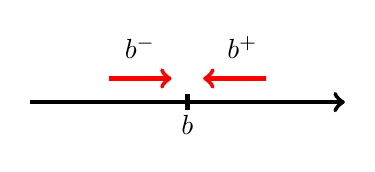
\begin{tikzpicture}
    \draw[->, ultra thick] (-2,0) -- (2,0);
    \foreach \x/\xtext in {0/$b$}
    \draw[ultra thick] (\x,0.5pt) -- (\x,-0.5pt) node[below] {\xtext};
    \draw[ultra thick] (0,-0.1) -- (0,0.1);
    \draw[{<-}, ultra thick, red] (0.2,0.3) -- (1,0.3);
    \draw[{->}, ultra thick, red] (-1,0.3) -- (-0.2,0.3);
    \node[label=$b^+$] at (0.7,0.3) {};
    \node[label=$b^-$] at (-0.6,0.3) {};
  \end{tikzpicture}
  \caption{Approaching to number b, from left: $b^-$ and from right: $b^+$}
\end{figure}


We might also have a situation when $x$ is decreasing or increasing without bound, meaning we are moving toward $-\infty$ or $+\infty$. In mathematics, we can express them like this:
\begin{itemize}
    \item Decreasing without bound: $x \rightarrow -\infty$
    \item Increasing without bound: $x \rightarrow +\infty$
\end{itemize}
%
\begin{figure}[ht]
  \centering
  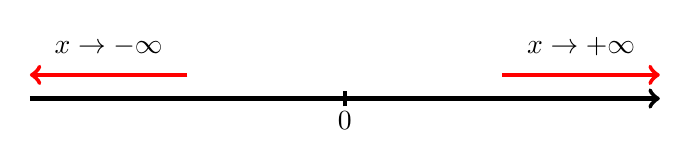
\begin{tikzpicture}
    \draw[->, ultra thick] (-4,0) -- (4,0);
    \foreach \x/\xtext in {0/$0$}
    \draw[ultra thick] (\x,0.5pt) -- (\x,-0.5pt) node[below] {\xtext};
    \draw[ultra thick] (0,-0.1) -- (0,0.1);
    \draw[{->}, ultra thick, red] (2,0.3) -- (4,0.3);
    \draw[{->}, ultra thick, red] (-2,0.3) -- (-4,0.3);
    \node[label=$x \rightarrow +\infty$] at (3,0.3) {};
    \node[label=$x \rightarrow-\infty$] at (-3,0.3) {};
  \end{tikzpicture}
  \caption{Decreasing and increasing without bound}
\end{figure}
%
Arrow notation is very important and useful, particularly in calculus when we need to use limit. You can find the summary of all arrow notations in the table below.
\begin{table}[ht]
  \centering
  \caption{Arrow Notations}
  \begin{tabular}{c|c}
    \toprule
    Arrow Notation & Meaning \\
    \hline \hline
    $x \rightarrow b^-$ & $x$ approaches to $b$ from left ($x<b$ but close to $b$) \\
    $x \rightarrow b^+$ & $x$ approaches to $b$ from right ($x>b$ but close to $b$) \\
    $x \rightarrow -\infty$ & $x$ approaches $-\infty$ ($x$ decreases without bound) \\    
    $x \rightarrow +\infty$ & $x$ approaches $+\infty$ ($x$ increases without bound) \\
    \bottomrule
  \end{tabular}
   \label{tab:arrow_notation}
\end{table}
% =============
\section{Reciprocal function}
Of many rational functions, reciprocal function defined as 
%
\begin{equation}
    f(x)=\frac{1}{x}
    \label{reciprocal_funct}
\end{equation}
%
is the most noteworthy. The domain of this function is all real number, except 0.
%
\begin{equation*}
    \text{Domain of a reciprocal function}: \{x \mid x\neq0\}
\end{equation*}
%
Let's plot the reciprocal function. Since $x=0$ is not in our domain, we begin by observing the behaviour of the graph around $x=0$.\\
If we move toward $0$ from left, i.e. $x \rightarrow 0^-$, we will notice the function gets bigger and bigger but in negative direction. On the other hand, if we approach to $0$ from right, i.e. $x \rightarrow 0^+$, function $f$ get bigger in positive direction. Using mathematical notation, we can say
%
\begin{itemize}
    \item If $x \rightarrow 0^-$, $f(x) \rightarrow -\infty$.
    \item If $x \rightarrow 0^+$, $f(x) \rightarrow +\infty$.
\end{itemize}
%
Table \ref{tab:reciprocal_zero} is showing this behavior. As you can see, $x=0$ is a pole that the $f$ never reaches to it, but when we get close to this pole, the $f$ goes to infinity.
\begin{table}[ht]
\centering
\caption{Function values around $x=0$}

\begin{tabular}{c|c}
    $x$ & $f(x)=\frac{1}{x}$ \\
    \\[-1em]
    \hline
    -1     & -1 \\
    -0.5   & -2 \\
    -0.1   & -10 \\
    -0.01  & -100 \\
    -0.001 & -1000 \\
    \vdots & \vdots
\end{tabular}
\qquad
\begin{tabular}{c|c}
    $x$ & $f(x)=\frac{1}{x}$ \\
    \\[-1em]
    \hline
    1     & 1 \\
    0.5   & 2 \\
    0.1   & 10 \\
    0.01  & 100 \\
    0.001 & 1000 \\
    \vdots & \vdots
\end{tabular}
\label{tab:reciprocal_zero}
\end{table}


Now let's see what will happen if $x$ decreases or increases without bound. If $x$ goes to negative infinity, we notice, the reciprocal function gets smaller and smaller. Likewise, if $x$ goes to positive infinity, we'll see the same behavior. Table \ref{tab:reciprocal_infinity} is showing this behavior when $x$ goes to infinity.
\begin{table}[ht]
\centering
\caption{Function values around when $x$ goes negative and positive infinity}

\begin{tabular}{c|c}
    $x$ & $f(x)=\frac{1}{x}$ \\
    \\[-1em]
    \hline
    -1     & -1 \\
    -2   & -0.5 \\
    -10   & -0.1 \\
    -100  & -0.01 \\
    -1000 & -0.001 \\
    \vdots & \vdots
\end{tabular}
\qquad
\begin{tabular}{c|c}
    $x$ & $f(x)=\frac{1}{x}$ \\
    \\[-1em]
    \hline
    1     & 1 \\
    2   & 0.5 \\
    10   & 0.1 \\
    100  & 0.01 \\
    1000 & 0.001 \\
    \vdots & \vdots
\end{tabular}
\label{tab:reciprocal_infinity}
\end{table}
As you can observe, As $x$ goes to infinity, whether positive or negative, $f$ will get close to a horizontal line $y=0$.\\
Using all of these information, we can graph the reciprocal function, shown in Figure \ref{fig:reciprocal}. 
\begin{figure}[ht]
\centering
 \begin{tikzpicture}
 \begin{axis}[
        my style,
        ytick=\empty,
        xtick=\empty,
        xmin=-3,xmax=3,ymin=-10,ymax=10, 
        samples=1000, 
        x label style={at={(axis description cs:1,0.5)},anchor=north},
        y label style={at={(axis description     cs:0.5,1)},anchor=south},
        thick]
        \addplot +[<->, mark=none, red, ultra thick, smooth, domain=-3:-0.1] (x,1/x);
        \addplot +[<->, mark=none, red, ultra thick, smooth, domain=0.1:3] (x,1/x);
        \node[text=red] at (2,3) {$f(x)=1/x$};
 \end{axis}
 \end{tikzpicture}
 \caption{The graph of the reciprocal function.}
 \label{fig:reciprocal}
\end{figure}
The pole $x=0$ is called \textbf{vertical asymptote}. Whereas,  the horizontal line $y=0$ is called \textbf{horizontal asymptote}. In next session, we will discuss how to find these two types of asymptotes. 
\begin{nt}
    There is also one more asymptote called \textbf{slant or oblique asymptote}. This type of asymptote appears in  some rational functions. In this case, when $x$ goes to infinity, $f$ approaches to a line, $y=mx+b$. We won't discuss this type of asymptote in this course.
\end{nt}
\begin{nt}
    Using the transformations, we can graph any different types of reciprocal functions. If we have $\displaystyle f(x)= \frac{a}{bx+h}+k$, then
    \begin{enumerate}
        \item \textbf{Shift horizontally}: Shift $h$ unit horizontally: right if $h<0$; left if $h>0$
        \item \textbf{Shrink or stretch horizontally}: Multiply all $x$-coordinates of function by $b$. If $b>1$, the graph will shrink and if $0<b<1$, the graph will stretch horizontally.
        \item \textbf{Shrink or stretch vertically}: Multiply all $y$-coordinates of function by $a$. If $a>1$, the graph will stretch and if $0<a<1$, the graph will stretch vertically.
        \item \textbf{Shift vertically}: Shift $k$ unit vertically: upward if $k>0$; downward of $k<0$.
    \end{enumerate}
\end{nt}
% =======
\begin{nt}
    We use dashed line to show vertical and horizontal asymptotes when we graph a rational function.
\end{nt}
% ========
\section{Vertical asymptotes}
The line $x = a$ is a vertical asymptote of the function $y = f(x)$ if $y$ approaches $\pm \infty$ as $x$ approaches $a$ from the right or left.\\
To find vertical asymptote, it is first important to simplify the rational function, meaning to factor both numerator and denominator and cancel out the common factors. Then we set the denominator to 0 and solve for $x$.
\begin{tcolorbox}[title= Vertical asymptote, fonttitle=\bfseries]
To find vertical asymptotes, follow these steps:
\begin{enumerate}[1.]
    \item Simplify the rational expression
    \item Set the denominator to 0 and solve for $x$
\end{enumerate}
\end{tcolorbox}
% ======== EXAMPLE
\begin{exa}
        Find the vertical asymptote(s) of following functions:
        \begin{equation*}
            f(x) = \frac{x+3}{x-5}
        \end{equation*}
\end{exa}
\begin{align*}
    \frac{x+3}{x-5}&     &   &\text{Simplfy fraction}\\
    \frac{1.(x+3)}{1.(x-5)}&    &   &\text{gcf of both numerator and denominator is $1$}\\
    &   &   &\text{No common factors! }\\
    x-5=0&    &   &\text{Set denominator to 0}\\
    x = 5&   &      &\text{Our vertical asymptote}
\end{align*}
The graph of this function is shown in Figure \ref{fig:ex_1}.
\begin{figure}[ht]
    \centering
    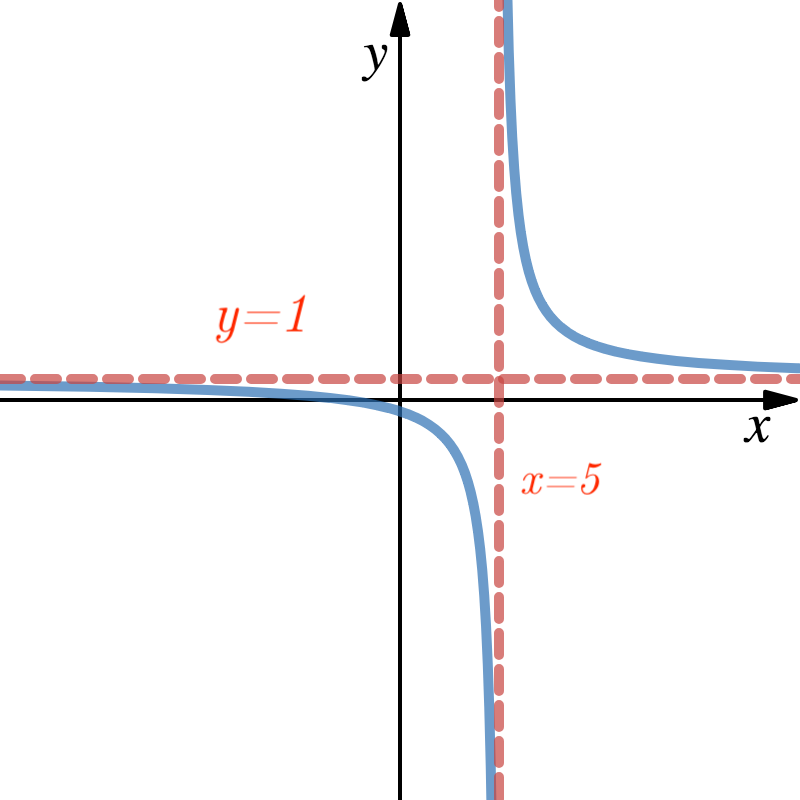
\includegraphics[width=7cm]{pics/ex1.png}
    \caption{The graph of $f(x)=\frac{x+3}{x-5}$. There is a vertical asymptote which is $x=5$. Also there is a horizontal one $y=1$}
    \label{fig:ex_1}
\end{figure}
% =========== NOTE
\begin{nt}
    Once a factor in the denominator got canceled out, zeros of that factor is not a vertical asymptote instead there will be a hole at that point. That's why it is very very important to simplify the rational function first and then set the denominator equal to 0. 
\end{nt}
% ===========
\begin{exa}
        Find the vertical asymptote of the following function:
        \begin{equation*}
             f(x) = \frac{x-5}{x^2-25}
        \end{equation*}
\end{exa}
\begin{align*}
    \frac{x-5}{x^2-25} &        &   &\text{Factor both numerator and denominator}\\
    \frac{1.\cancel{(x-5)}}{\cancel{(x-5)}(x+5)}&     &   &\text{Cancel out $x-5$}\\
    \frac{1}{x+5}&      &   &\text{Now set the denominator to 0}\\
    x+5=0&      &   &\text{Solve for $x$}\\
    x = -5&     &   &\text{Our vertical asymptote}
\end{align*}
Notice, factor $x-5$ got cancelled out during simplification step. Zero of this factor is $x=5$. At this point, we will have a hole in our graph instead of vertical asymptote, as shown in Figure \ref{fig:ex_2}
\begin{figure}[ht]
    \centering
    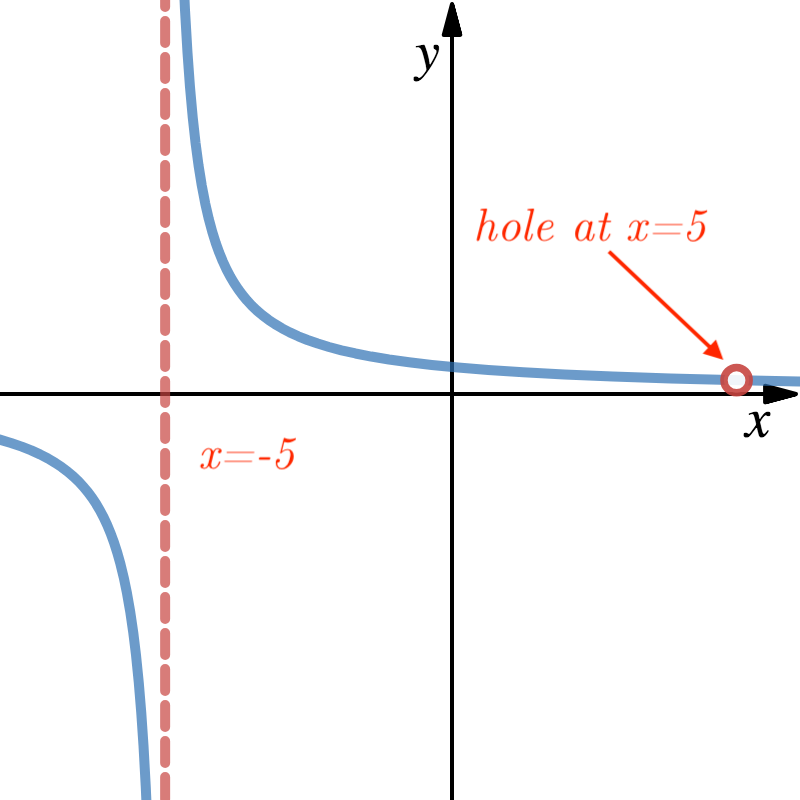
\includegraphics[width=7cm]{pics/ex2.png}
    \caption{The graph of $f(x)=\frac{x-5}{x^2-25}$. There is only one vertical asymptote at $x=-5$. At $x=-5$, there is a hole in graph because it is not in our domain and it not a vertical asymptote as well.}
    \label{fig:ex_2}
\end{figure}
% ===========
\begin{exa}
        Find the vertical asymptote of the following function:
        \begin{equation*}
                    f(x) = \frac{x^2+1}{x^2+x-6}
        \end{equation*}
\end{exa}
\begin{align*}
    \frac{x^2+1}{x^2+x-6}&      &   &\text{Factor out both numerator and denominator}\\
    \frac{1.(x^2+1)}{(x-2)(x+3)}&   &   &\text{No common factor!}\\
    (x-2)(x+3)=0&       &       &\text{Set the denominator equal to 0}\\
    x=2&    &   &\text{First vertical asymptote}\\
    x=-3&   &   &\text{Second vertical asymptote}
\end{align*}
As you can see, in this example we have more than 1 vertical asymptote. The graph of this function is shown in Figure \ref{fig:ex_3}.
\begin{figure}[ht]
    \centering
    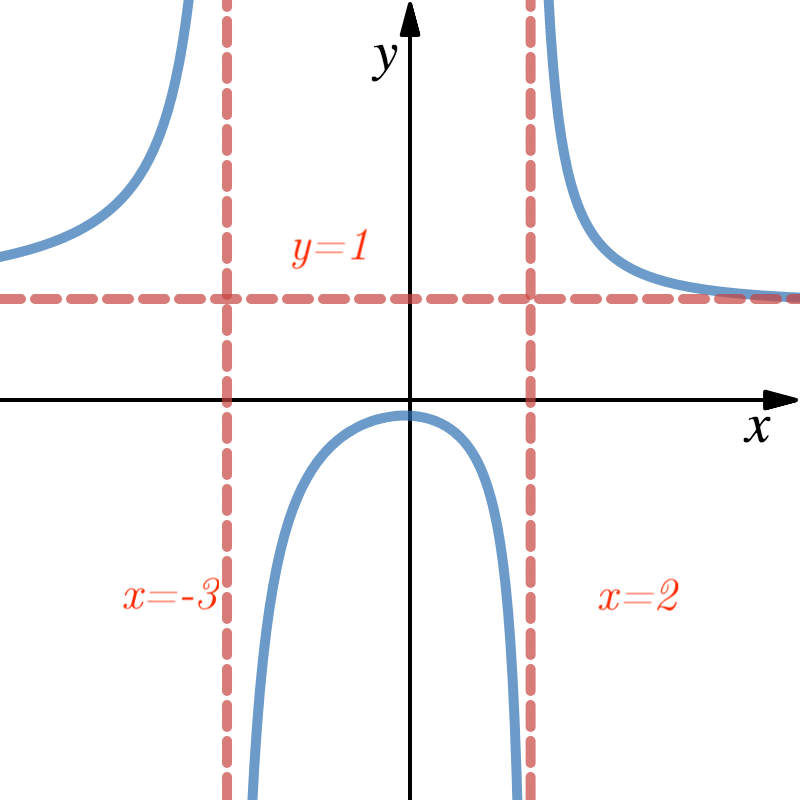
\includegraphics[width=7cm]{pics/ex3.png}
    \caption{The graph of $f(x)=\frac{x^2+1}{x^2+x-6}$. There are two vertical asymptotes, $x=-3$ and $x=2$. There is also a horizontal asymptote $y=1$.}
    \label{fig:ex_3}
\end{figure}
% ======== SECTION
\section{Horizontal asymptote}
The line $y = b$ is a horizontal asymptote of the function $y = f(x)$ if $y$ approaches $b$ as $x$ approaches $\pm \infty$.\\
To find the horizontal asymptote, degree of numerator and denominator play an important role. Let $f(x)$ be:
\begin{equation*}
        f(x)=\frac{a_1x^n+a_2x^{n-1}+\ldots}{b_1x^m+b_2x^{m-2}+\ldots}
\end{equation*}
The degree of numerator is $n$ and degree of denominator is $m$. The leading coefficient of numerator is $a_1$ and the leading coefficient of denominator is $b_1$.
\begin{enumerate}[I.]
    \item If $n=m$, then there is one horizontal asymptote at $y= \frac{a_1}{b_1}$.
    \item If $n<m$, then there is one horizontal asymptote at $y= 0$.
    \item If $n>m$, we don't have any horizontal asymptote.
\end{enumerate}
% ======= EXAMPLE
\begin{exa}
        Find the horizontal asymptote of each functions:
        \begin{enumerate}[\bfseries a.]
            \item $f(x)=\frac{4x^3-2x+1}{2x^3-2x^2+10}$
            \item $f(x)=\frac{3x-4}{6x^2+2x-1}$
            \item $f(x)=\frac{7x^2-1}{x+5}$
        \end{enumerate}
\end{exa}
Let $n$ degree of numerator and $m$ degree of denominator.\\
a.
\begin{align*}
    \frac{4x^3-2x+1}{2x^3-2x^2+10}&     &   &\text{$n=3$ and $m=3$ so $n=m$}\\
    \frac{\circled{4}x^3-2x+1}{\circled{2}x^3-2x^2+10}&    &
    &\text{Case I, divide leading coefficients}\\
    y=\frac{4}{2}=2&    &   &\text{Our horizontal asymptote}
\end{align*}
\\[0.2cm]
b.
\begin{align*}
    \frac{3x-4}{6x^2+2x-1}&     &   &\text{$n=1$ and $m=6$ so $n<m$}\\
    \frac{3x-4}{6x^2+2x-1}&    &  &\text{Case II}\\
    y=0&    &   &\text{Our horizontal asymptote}
\end{align*}
\\[0.2cm]
c.
\begin{align*}
    \frac{7x^2-1}{x+5}&     &   &\text{$n=2$ and $m=1$ so $n>m$}\\
    \frac{7x^2-1}{x+5}&    &  &\text{Case III}\\
    \xmark&    &   &\text{No horizontal asymptote}
\end{align*}